\section{1174086 - Tia Nur Candida}

\subsection{Teori}
\begin{enumerate}
\item Binary Classification \\
Binary Classification, yang berarti mengklasifikasikan objek dari suatu himpunan menjadi dua kelompok, tetapi teknik ada untuk klasifikasi multikelas.

\hfill\break
\begin{figure}[H]
    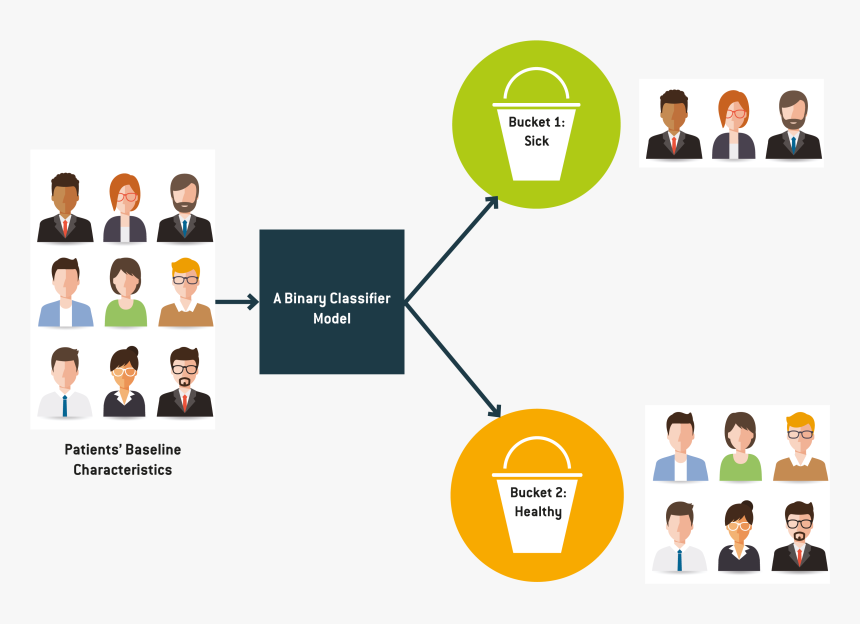
\includegraphics[width=6cm]{figures/1174086/2/binary.png}
    \centering
    \caption{Binary Classification}
\end{figure}

\item Supervised Learning, Unsupervised Learning dan Clustering \\
\begin{itemize}
\item Supervised Learning \\
supervised learning mempuyai input dan output yang dapat dibuat menjadi suatu model hubungan matematis sehingga mampu melakukan prediksi dan klasifikasi berdasarkan data yang telah ada sebelumnya. supervised learning membutuhkan data training agar mampu melakukan prediksi maupun klasifikasi. supervised learning, algoritma tersebut seolah-olah dilatih terlebih dahulu agar dapat melakukan prediksi maupun klasifikasi.
\begin{figure}[H]
    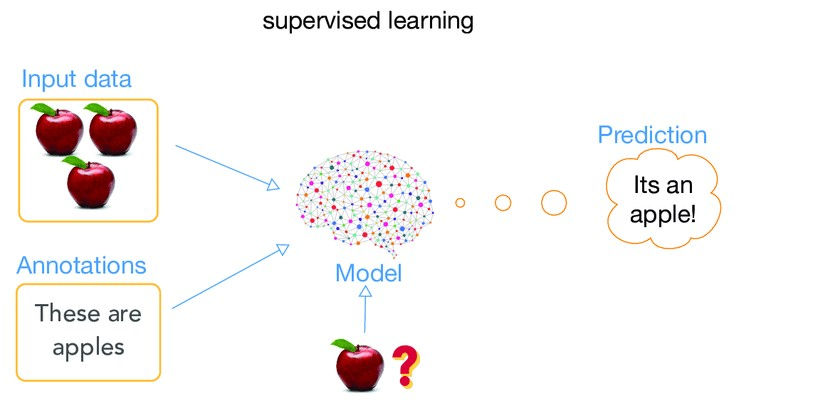
\includegraphics[width=6cm]{figures/1174086/2/super.jpg}
    \centering
    \caption{Supervised Learning}
\end{figure}

\item Unsupervised Learning \\
Unsupervised learning tidak menggunakan data latih atau data training untuk melakukan prediksi maupun klasifikasi. Berdasarkan model matematisnya, algoritma ini tidak memiliki target variabel. Salah satu tujuan dari algoritma ini adalah mengelompokkan objek yang hampir sama dalam suatu area tertentu.
\begin{figure}[H]
    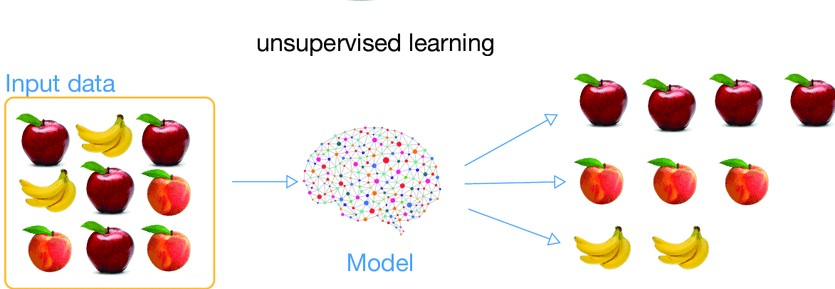
\includegraphics[width=6cm]{figures/1174086/2/un.jpg}
    \centering
    \caption{Unsupervised Learning}
\end{figure}

\item Clustering \\
Teknik clustering ini masuk ke dalam kelompok unsupervised learning, yang artinya ini merupakan teknik di mana mesin akan bekerja (belajar) sendiri tanpa kita ajari bagaimana cara memecahkan permasalahannya.
Sebagai contoh, anggap saja kita memiliki sebuah data, misal data pelanggan yang berisi tentang jenis kelamin, besarnya penghasilan dan besarnya pembelian produk-produk kita. Maka dengan algoritma clustering kita dapat mengetahui pelanggan kita akan dikelompokkan ke dalam beberapa kluster dengan sendirinya, misal ada pelanggan yang pelit, pelanggan yang royal dan lain sebagainya.

\hfill\break
\begin{figure}[H]
    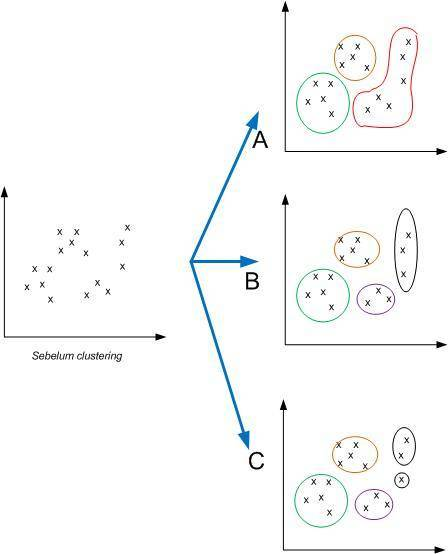
\includegraphics[width=4cm]{figures/1174086/2/clustering.jpg}
    \centering
    \caption{Clustering}
\end{figure}

Ada 3 hasil klustering, yaitu A (menjadi 3 kluster), B (menjadi 4 kluster) dan C (menjadi 5 kluster). Manakah yang paling baik pembagiannya? Apakah A, B atau C? Itu semua tergantung kita sebagai pembuat algoritmanya. Jika kita menginginkan 3 kluster saja, maka mungkin A yang terbaik. Jika kita ingin 5 dan sangat detail, maka C yang terbaik. Itupun juga tergantung bagaimana data yang kita miliki.

\end{itemize}

\item Evaluasi dan Akurasi \\
Evaluasi adalah kegiatan yang dilakukan berkenaan dengan proses untuk menentukan nilai dari suatu hal.
Kita dapat mengevaluasi seberapa baik model bekerja dengan mengukur akurasinya. 
Akurasi akan didefinisikan sebagai persentase kasus yang diklasifikasikan dengan benar.

\begin{figure}[H]
    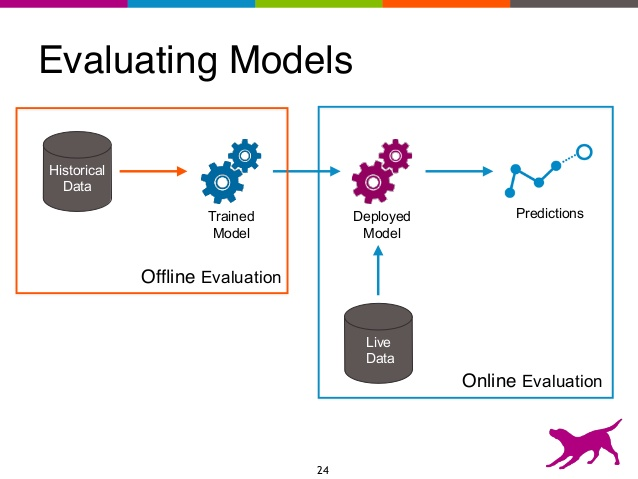
\includegraphics[width=4cm]{figures/1174086/2/eva.jpg}
    \centering
    \caption{Evaluation}
\end{figure}
\begin{figure}[H]
    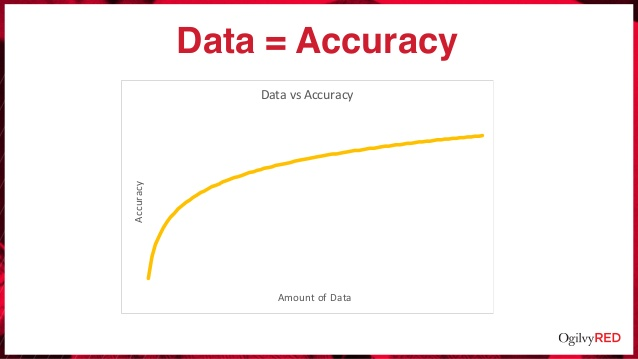
\includegraphics[width=4cm]{figures/1174086/2/acc.jpg}
    \centering
    \caption{Accuracy}
\end{figure}
\item Confusion Matrix \\
Confusion matrix juga sering disebut error matrix. Pada dasarnya confusion matrix memberikan informasi perbandingan hasil klasifikasi yang dilakukan oleh sistem (model) dengan hasil klasifikasi sebenarnya. Confusion matrix berbentuk tabel matriks yang menggambarkan kinerja model klasifikasi pada serangkaian data uji yang nilai sebenarnya diketahui.
Terdapat 4 istilah sebagai representasi hasil proses klasifikasi pada confusion matrix
\begin{itemize}
\item True Positive (TP)
Merupakan data positif yang diprediksi benar. Contohnya, pasien menderita kanker (class 1) dan dari model yang dibuat memprediksi pasien tersebut menderita kanker (class 1).
\item True Negative (TN)
Merupakan data negatif yang diprediksi benar. Contohnya, pasien tidak menderita kanker (class 2) dan dari model yang dibuat memprediksi pasien tersebut tidak menderita kanker (class 2).
\item False Postive (FP) — Type I Error
Merupakan data negatif namun diprediksi sebagai data positif. Contohnya, pasien tidak menderita kanker (class 2) tetapi dari model yang telah memprediksi pasien tersebut menderita kanker (class 1).
\item False Negative (FN) — Type II Error
Merupakan data positif namun diprediksi sebagai data negatif. Contohnya, pasien menderita kanker (class 1) tetapi dari model yang dibuat memprediksi pasien tersebut tidak menderita kanker (class 2).
\begin{figure}[H]
    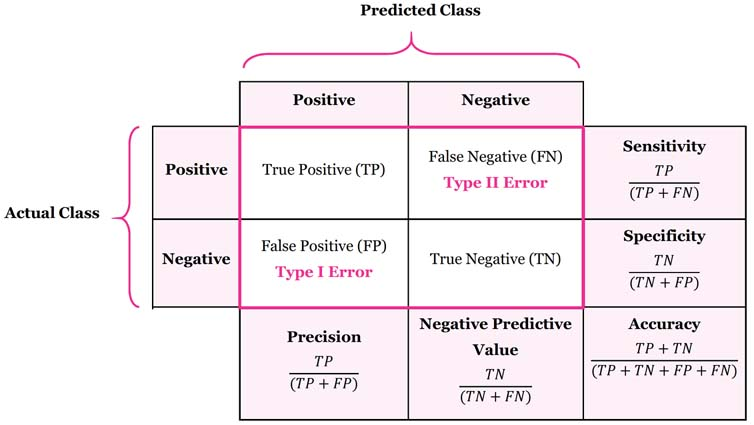
\includegraphics[width=8cm]{figures/1174086/2/confmat.jpg}
    \centering
    \caption{Confussion Matrix}
\end{figure}


\end{itemize}
\item K-Fold 

Cara kerja k-fold validation:
\begin{itemize}
	\item Total instance dibagi menjadi N bagian.
	\item Fold yang pertama adalah bagian pertama menjadi data uji (testing data) dan sisanya menjadi training data.
	\item Lalu hitung akurasi berdasarkan porsi data tersebut dengan menggunakan persamaan.
	\item Fold yang kedua adalah bagian kedua, yang menjadi data uji(testing data)dan sisanya training  data.
	\item Kemudian hitung akurasi berdasarkan porsi data tersebut.
	\item Dan seterusnya hingga habis mencapai fold ke-K.
	\item Terakhir hitung rata-rata akurasi K buah.
\end{itemize}
\begin{figure}[H]
    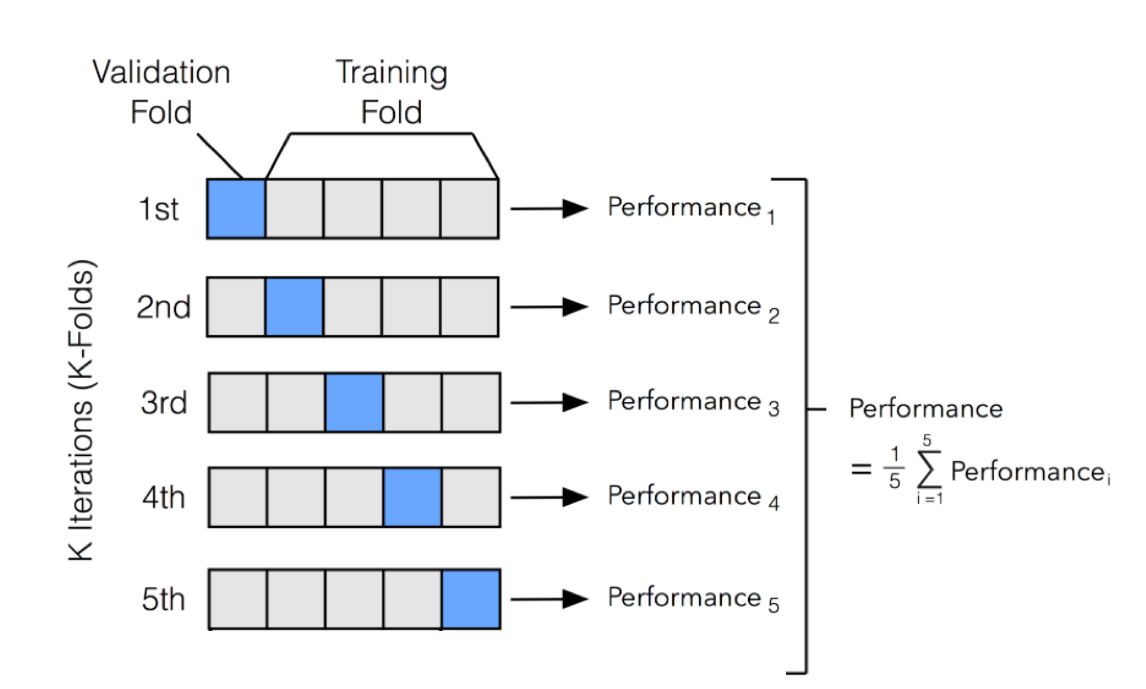
\includegraphics[width=8cm]{figures/1174086/2/kfolds.png}
    \centering
    \caption{contoh K-Fold Validation}
\end{figure}
\item Decision Tree \\
Decision tree adalah salah satu metode klasifikasi yang paling populer, karena mudah untuk diinterpretasi oleh manusia. Decision tree adalah model prediksi menggunakan struktur pohon atau struktur berhirarki. Konsep dari pohon keputusan adalah mengubah data menjadi decision tree dan aturan-aturan keputusan.
\begin{figure}[H]
    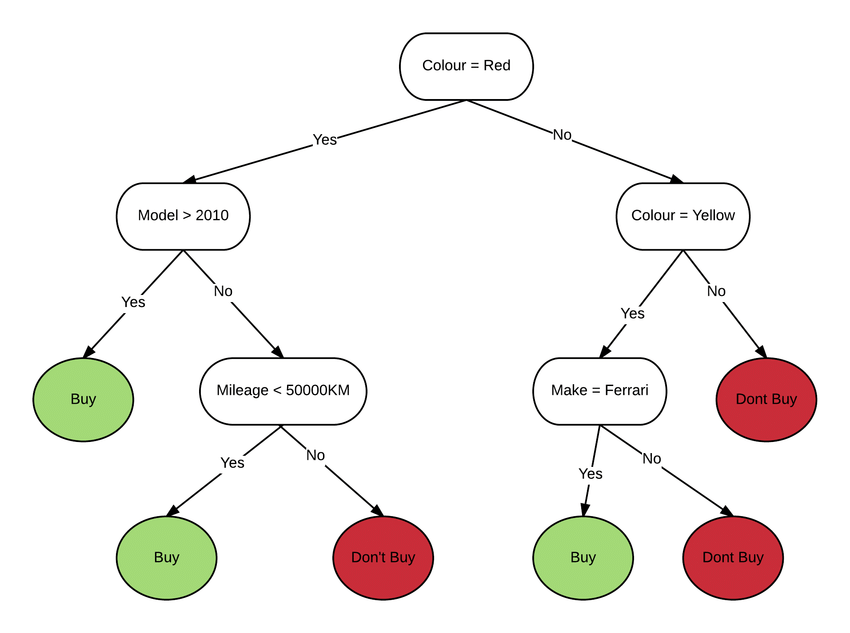
\includegraphics[width=8cm]{figures/1174086/2/decisiontree.png}
    \centering
    \caption{Decision Tree}
\end{figure}
\item Entropy dan Information Gain \\
Algoritma pada metode ini menggunakan konsep dari entropi. Konsep Entropi yang digunakan untuk mengukur “seberapa informatifnya” sebuah node (yang biasanya disebut seberapa baiknya).\\
Entropi adalah nilai informasi yang menyatakan ukuran ketidakpastian (impurity) dari attribut dari suatu kumpulan obyek data dalam satuan bit.\\
Information Gain adalah ukuran efektifitas suatu atribut dalam mengklasifikasikan data. Digunakan untuk menentukan urutan atribut dimana attribut yang memiliki nilai Information Gain terbesar yang dipilih

\begin{figure}[H]
    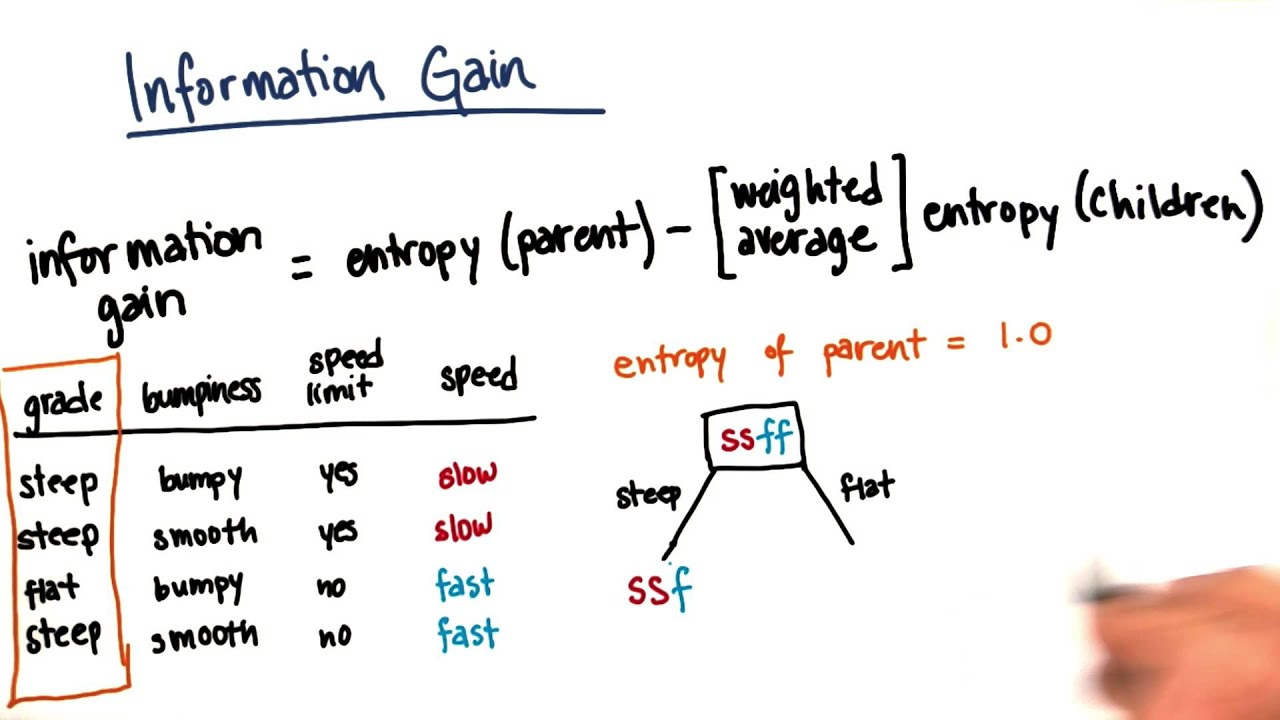
\includegraphics[width=8cm]{figures/1174086/2/en.jpg}
    \centering
    \caption{Information Gain}
\end{figure}




\end{enumerate}


\subsection{Praktek}

\hfill\\
\lstinputlisting[firstline=8, lastline=110]{src/1174086/2/chp2.py}


\subsection{Penanganan Error}
\begin{enumerate}
\item Screenshoot Error

\begin{figure}[H]
		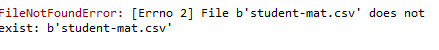
\includegraphics[width=4cm]{figures/1174086/2/error/error1.PNG}
		\centering
		\caption{File Not Found}
	\end{figure}
	
	\begin{figure}[H]
		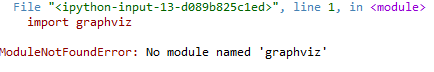
\includegraphics[width=4cm]{figures/1174086/2/error/error2.PNG}
		\centering
		\caption{Module Not Found}
	\end{figure}
	
	\begin{figure}[H]
		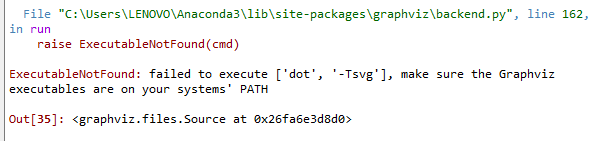
\includegraphics[width=4cm]{figures/1174086/2/error/error3.PNG}
		\centering
		\caption{Executable Not Found}
	\end{figure}
	
\item Jenis Error
	\begin{itemize}
	\item File Not Found
	\item Module Not Found
	\item Executable Not Found
	\end{itemize}
	
\item Solusi Error
\begin{itemize}
	\item File Not Found\\
	Mendownload filenya di github
	\begin{figure}[H]
		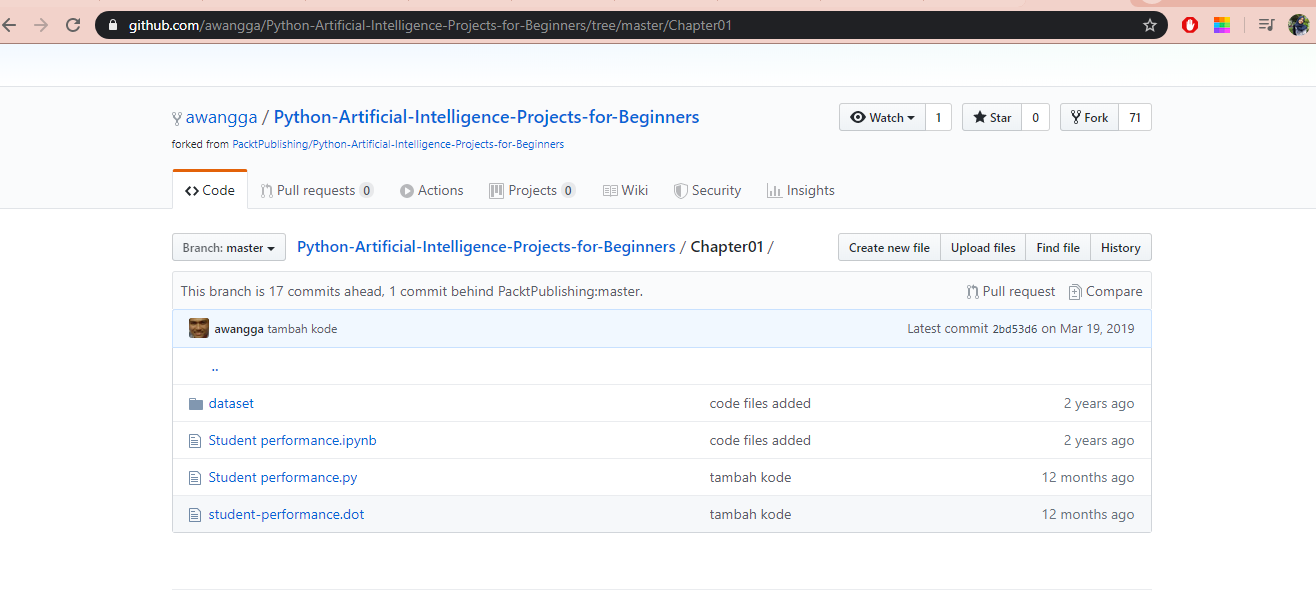
\includegraphics[width=4cm]{figures/1174086/2/error/solusi1.PNG}
		\centering
		\caption{File Dataset}
	\end{figure}
	
	\item Module Not Found\\
	Mendownload library graphviz menggunakan pip install graphviz di Anaconda Prompt
	\begin{figure}[H]
		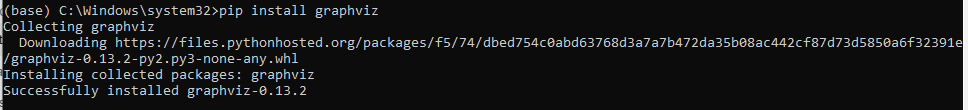
\includegraphics[width=4cm]{figures/1174086/2/error/solusi2.PNG}
		\centering
		\caption{Install graphviz}
	\end{figure}
	
	\item Executable Not Found
	
	\end{itemize}
\end{enumerate}


\subsection{Bukti Tidak Plagiat}
\begin{figure}[H]
	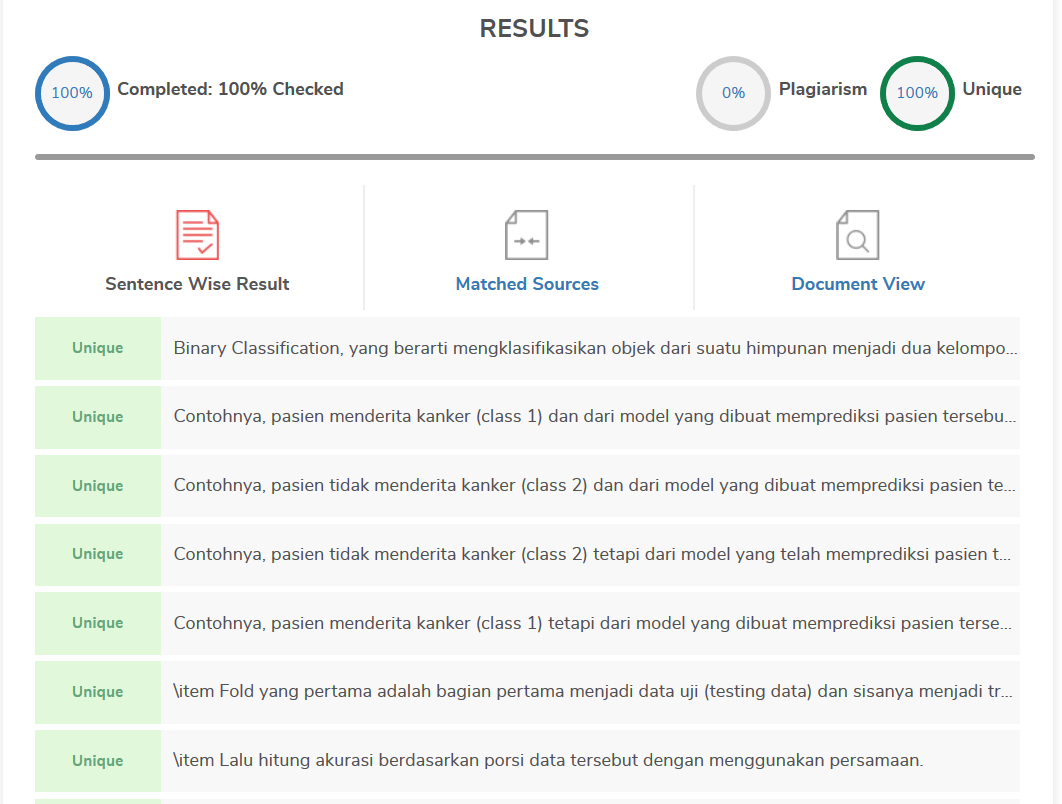
\includegraphics[width=4cm]{figures/1174086/2/plagiarisme.PNG}
	\centering
	\caption{Bukti Tidak Plagiat}
\end{figure}